% Offizielle Beispieldatei für beamer-Vorlage aus tubslatex Version 0.3beta2
\documentclass[fleqn,11pt,aspectratio=43]{beamer}

\usepackage[ngerman]{babel}
\usepackage[utf8x]{inputenc}
\usepackage{graphicx}
\usetheme[%
  %nexus,%        Nexus Fonts benutzen
  %lnum,%         Versalziffern verwenden
  %cmyk,%<rgbprint>,          Auswahl des Farbmodells
  blue,%<orange/green/violet> Auswahl des Sekundärfarbklangs
  dark,%<light,medium>        Auswahl der Helligkeit
  %colorhead,%    Farbig hinterlegte Kopfleiste
  %colorfoot,%    Farbig hinterlegt Fußleiste auf Titelseite
  colorblocks,%   Blöcke Farbig hinterlegen
  %nopagenum,%    Keine Seitennumer in Fußzeile
  %nodate,%       Kein Datum in Fußleiste
  tocinheader,%   Inhaltsverzeichnis in Kopfleiste
  %tinytocinheader,% kleines Kopfleisten-Inhaltsverzeichnis
  %widetoc,%      breites Kopfleisten-Inhaltsverzeichnis
  %narrowtoc,%    schmales Kopfleisten-Inhaltsverzeichnis
  %nosubsectionsinheader,%  Keine subsections im Kopfleisten-Inhaltsverzeichnis
  %nologoinfoot,% Kein Logo im Fußbereich darstellen
  ]{tubs}

% Titelseite
\title{Meine Pr\"asentation}
\subtitle{Das Corporate Design in  \LaTeX}
\author{Max Mustermann}
% Titelgrafik, automatisch beschnitten, Weitere Optionen: <scaled/cropx/cropy>
% \titlegraphic[cropped]{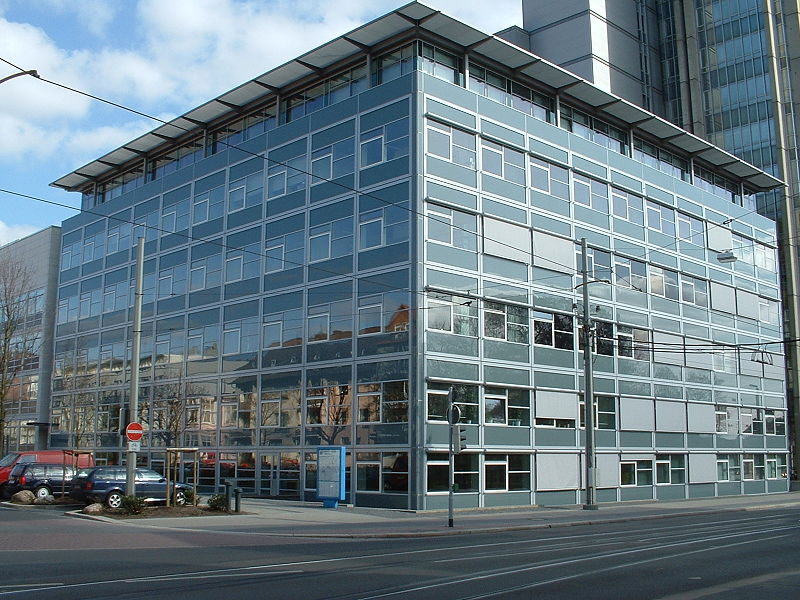
\includegraphics{infozentrum.jpg}}
\titlegraphic[scaled]{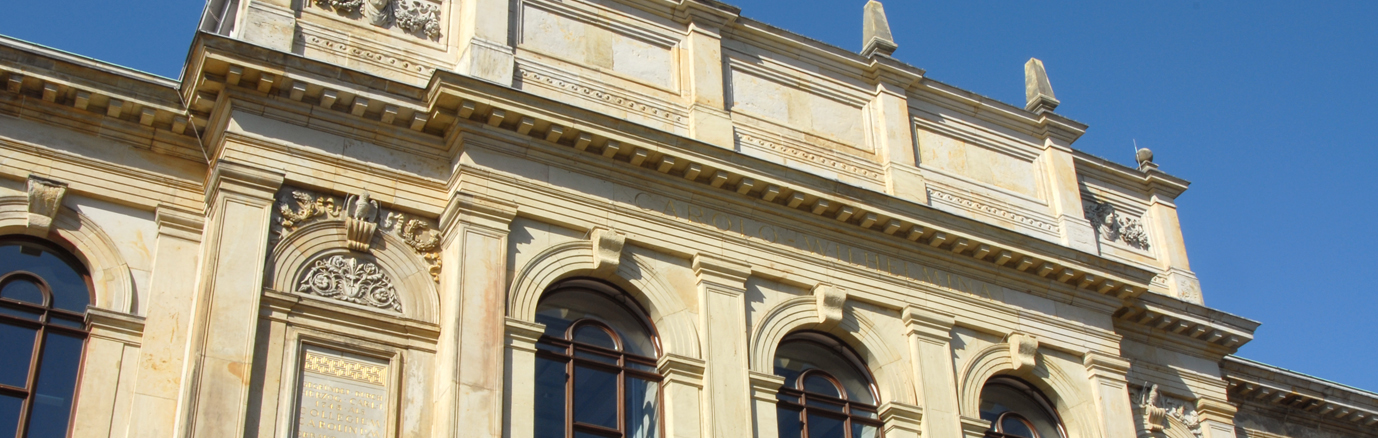
\includegraphics{titlepicture.jpg}}

% Logo, dass auf Titelseiten oben rechts und auf Inthaltsseiten unten rechts
% dargestellt wird. Es wird jeweils automatisch skliert
\logo{
\includegraphics{dummy_institut.pdf}}
%\logo{Institut für Unkreativität\\und Schreibschwäche}
\date{01.01.1970}

\begin{document}

\begin{frame}[plain]
\titlepage
\end{frame}

\part{Erster Teil}

\begin{frame}[plain]
  \partpage
\end{frame}


\section{Kapitel 1}

\begin{frame}{Inhalt}
\tableofcontents
\end{frame}

\begin{frame}{Hier steht der Titel der Folie}
Wir beginnen mit einer Aufzählung
\begin{itemize}
  \item Aufzählzeichen werden als Quadrate dargestellt
  \begin{itemize}
    \item Unterpunkte ebenfalls
    \item Allerdings etwas kleiner
  \end{itemize}
\end{itemize}
\end{frame}

\section{Kapitel 2}


\begin{frame}{Itemize-Test}
  \begin{itemize}
    \item Lorem ipsum dolor sit amet, consetetur sadipscing elitr, sed diam
      nonumy eirmod tempor invidunt ut labore et dolore magna aliquyam
    \item At vero eos et accusam et justo duo dolores et ea rebum.
      \begin{itemize}
        \item Stet clita kasd gubergren, no sea takimata sanctus est Lorem ipsum
          dolor sit amet!
          \begin{itemize}
            \item Nam eget dui.
            \item Maecenas tempus, tellus eget condimentum rhoncus, sem quam
              semper libero, sit amet adipiscing sem neque sed ipsum.
          \end{itemize}
        \item Duis leo
      \end{itemize}
    \item Aliquam lorem ante, dapibus in, viverra quis, feugiat a, tellus. 
  \end{itemize}
\end{frame}


\subsection{Unterkapitel 1}


\begin{frame}{Mathe-Test}
  Gaußsche Summenformel:
  \[1 + 2 + 3 + 4 + \ldots + n = \sum_{k=1}^n k = \frac{n(n+1)}{2}\]
  Faltung:
  \[(f*g)(\xi) := \int_{\mathbb{R}^n} f(y)g(\xi-y)\mathrm{d}y\]
\end{frame}


\part{Zweiter Teil}


\begin{frame}
  \partpage
\end{frame}


\section{Ende}


\begin{frame}{Farbklänge}\small
  Farbklänge tuOrange\ldots, tuBlue\ldots, tuGreen\ldots, tuViolet\ldots\\\tiny
  \colorshow[0.95\textwidth]{Orange}{Dark}%
  \colorshow[0.95\textwidth]{Orange}{Medium}%
  \colorshow[0.95\textwidth]{Orange}{Light}~\\
  \colorshow[0.95\textwidth]{Blue}{Dark}%
  \colorshow[0.95\textwidth]{Blue}{Medium}%
  \colorshow[0.95\textwidth]{Blue}{Light}~\\
  \colorshow[0.95\textwidth]{Green}{Dark}%
  \colorshow[0.95\textwidth]{Green}{Medium}%
  \colorshow[0.95\textwidth]{Green}{Light}~\\
  \colorshow[0.95\textwidth]{Violet}{Dark}%
  \colorshow[0.95\textwidth]{Violet}{Medium}
  \colorshow[0.95\textwidth]{Violet}{Light}
\end{frame}


\begin{frame}{Farbtest}
  \color{tuRed}
  Dies ist ein Text in tuRed.

  \color{tuSecondaryDark80}
  Dies ist ein Text in tuSecondaryDark80.

  \color{tuSecondaryLight}
  Dies ist ein Text in tuSecondaryLight.
\end{frame}


\begin{frame}{Verwendung von Spalten}
  \begin{columns}[onlytextwidth]
    \column{0.5\textwidth}
      Dies ist die erste Spalte.
      Die Angabe der Option \texttt{[onlytextwidth]}
      sorgt dafür, dass die Spaltenbreite korrekt eingehalten wird.
    \column{0.5\textwidth}
      Dies ist die zweite Spalte mit weiteren Informationen.
  \end{columns}
\end{frame}


\begin{frame}{Blöcke}
  \begin{block}{Diest ist ein Block}
    Lorem ipsum dolor sit amet, consetetur sadipscing elitr, sed diam
    nonumy eirmod tempor invidunt ut labore et dolore magna aliquyam
  \end{block}
  \begin{exampleblock}{Diest ist ein Example-Block}
    Lorem ipsum dolor sit amet, consetetur sadipscing elitr, sed diam
    nonumy eirmod tempor invidunt ut labore et dolore magna aliquyam
  \end{exampleblock}
  \begin{alertblock}{Diest ist ein Alert-Block}
    Lorem ipsum dolor sit amet, consetetur sadipscing elitr, sed diam
    nonumy eirmod tempor invidunt ut labore et dolore magna aliquyam
  \end{alertblock}
\end{frame}


\begin{frame}[fragile]{Quellcode}
Quellcode-Frames müssen immer die Option \texttt{[fragile]} tragen.
  \begin{verbatim}
#include <iostream>

using namespace std;

int main() {
  cout << "Hello World!";
}
  \end{verbatim}
\end{frame}


\begin{frame}[highlight]{Wichtig}
Diese Folie ist wichtig!
\end{frame}

\end{document}
